\documentclass[a5paper,9pt]{book}     % 
\usepackage[utf8]{inputenc}            % for input encoding
\usepackage{amsmath,amsfonts,amssymb}  % for mathematical symbols and fonts
\usepackage{tcolorbox}
\usepackage{caption}    % Package for better captions
\usepackage{eso-pic}     % Allows adding elements to the page background
\usepackage{graphicx}    % For including images
\usepackage{afterpage}   % To control background images after specific pages
\usepackage{listings}
\lstset{
    language=Python,        % Set language to Python
    showstringspaces=false  % Prevent spaces from being printed as visible characters
}

\usepackage[colorlinks=false]{hyperref}
\usepackage{footnotebackref}
\usepackage[hang, flushmargin]{footmisc}
\usepackage[a5paper, margin=0cm]{geometry} % for page layout
\usepackage{natbib}                    % for bibliography management
\usepackage{setspace}                  % for controlling line spacing
\usepackage{xcolor}

% Additional packages for consistent layout
\usepackage{fancyhdr}  % For custom headers and footers
\pagestyle{fancy}      % Set the page style to fancy
\fancyhf{}             % Clear all header and footer fields
\fancyhead[LE,RO]{\thepage} % Page numbers on the outer side
\fancyhead[LO,RE]{\nouppercase{\leftmark}} % Chapter titles in headers


% Define colors
\definecolor{comment}{rgb}{0.0, 0.5, 0.0} % A darker green
\definecolor{white}{rgb}{1.0, 1.0, 1.0}

\geometry{
    a5paper,         % Set the paper size to A5
    inner=15mm,      % Inner margin for binding (reduced from 25mm)
    outer=12mm,      % Outer margin (reduced from 20mm)
    top=15mm,        % Top margin (reduced from 25mm)
    bottom=12mm,     % Bottom margin (reduced from 20mm)
    headsep=7mm,     % Space between header and text (proportional to A5)
    footskip=7mm,    % Space between footer and text (proportional to A5)
    includehead,     % Include header in margin calculations
    includefoot,     % Include footer in margin calculations
}

% Command to set the background image for a single page
\newcommand\BackgroundPicFrontPage{
  \AddToShipoutPictureBG*{
    \AtPageLowerLeft{
      
\includegraphics[width=\paperwidth,height=\paperheight]{assets/background-frontpage.png}
    }
  }
}

% Switch to monospace font globally
\renewcommand{\familydefault}{\ttdefault}

% \doublespacing  % Use 1.5 line spacing
\setcounter{secnumdepth}{3}            % number sub-subsections
\setcounter{tocdepth}{0}               % depth of table of contents


% Prevent overflow issues
\setlength{\emergencystretch}{3em} % Allow slight stretching of lines
\sloppy                      % Loosen word spacing rules slightly
\widowpenalty=10000          % Avoid widow lines (single lines at the top of a page)
\clubpenalty=10000           % Avoid club lines (single lines at the bottom of a page)
\brokenpenalty=10000         % Avoid page breaks inside paragraphs
\raggedbottom                % Avoid stretching the page vertically

% Font and text spacing adjustments
\usepackage{microtype}       % Improves justification and spacing


\begin{document}

% Set the front page background image
\BackgroundPicFrontPage

\title{\textbf{There is a closed door at the end of the corridor}}
\author{\textbf{Mauricio van der Maesen de Sombreff}}
\date{\the\year}

\maketitle     % generate the title page

% Reset color after front page
\ClearShipoutPicture
\color{black}

% \clearpage  % Move to the next page (to avoid background on TOC)
\pagestyle{empty}  % No page number on the TOC
{
    \newgeometry{
        a5paper,         % Set the paper size to A5
        inner=15mm,      % Inner margin for binding (reduced from 25mm)
        outer=12mm,      % Outer margin (reduced from 20mm)
        top=2mm,        % Top margin (reduced from 25mm)
        bottom=12mm,     % Bottom margin (reduced from 20mm)
        headsep=2mm,     % Space between header and text (proportional to A5)
        footskip=7mm,    % Space between footer and text (proportional to A5)
        includehead,     % Include header in margin calculations
        includefoot,     % Include footer in margin calculations
    }  
    \small 
    \tableofcontents
    \normalsize
    \clearpage % Ensure new page for subsequent content
    \restoregeometry % Restore original margins
}

% \pagestyle{empty}  % No page number on the TOC

\newpage  % Move to the next page after TOC
\pagestyle{plain}  % Start page numbering again

\chapter*{preface}
\addcontentsline{toc}{chapter}{preface}
\normalsize

\newpage  % Move to the next page
The title for this thesis comes from an early memory. Without an abundance of organized memories, I still maintain a clear mental image of this corridor. It belongs to a first period of separation from reality, a generator of narratives intended to build sense. Building backwards the parameters for a Markov chain to generate the time sequence that predicts and explains the present.    

The title sets up a journey of exploration, with a hidden aspect, and the intention of uncovering it. The story ( if there is any ) {r}evolves around what is behind the door, why it is closed, and what it means as a memory.

The corridor leading to the closed door is a path of self-discovery and confrontation of personal fears. It implies a setting that is limiting and confined, adding to an atmosphere of tension lived in Uruguay until the restoration of democracy in 1985. The closed door is the focal point of such tension. It represents a barrier between protection and isolation, between reality and imagination, history and fiction.

In this context, I explore the themes of curiosity, the fear of the unknown, and a tendency to be constantly drawn toward the off-limits. What is the dark if not a manifestation of the unknown? It's a driving force for widening the senses and understanding the environment.

This book is the reflection of my current ongoing introspection, an exploration of the negative space of the memory, and an attempt to confront possible pasts in possible realities. As explored by Roland Barthes in his essay "The death of the author"\citep{barthes1967}, meaning in this thesis arises from intertextual relationships between chapters and ideas. 



This book is written in \LaTeX{} (\href{https://www.tug.org/texlive/quickinstall.html}{tug.org}) and managed as code. The scripts and fragments that compile into this text are available through the following link: 

\href{https://github.com/n2048-creative-technology/thesis}{https://github.com/n2048-creative-technology/thesis}.
\chapter*{introduction}
\addcontentsline{toc}{chapter}{introduction}
\begin{center}
\vspace{2cm}
\begin{flushright}
\footnotesize 
\lstinputlisting[language=Python]{quine.py}
\end{flushright}
\vspace{2cm}
\end{center}
\normalsize

\newpage  % Move to the next page
% talk about molds.
There is stubbornness in the craft of casting materials through mold making, despite how rewarding it can be. Its whole process makes it hard to allow for later changes. The mold is not the memory of a piece, nor its essence, but it will define its final shape. Is the environment in which we grow and develop ourselves such a kind of mold? 

I remember only fragments about my own past, but I've spent the last few years making stronger efforts to understand the ways in which I perceive my own "umwelt", why I react, and what I react to.  What shaped this current way of thinking? Without an objective memory of my own history, creating versions of this multidimensional mold in which I've cast my way of perceiving has become an iterative process of re-creation.

{\scriptsize \textcolor{comment}{\% recursive alterations allow for a progressive reshaping of perception. }}

The small snippet of code under the title of this chapter is called a Quine. It is a program that produces its own source code as output, exemplifying a form of computational self-reference. 

{\scriptsize \textcolor{comment}{\% The quine and implies a connection between software, computer models and a human tendency for self-replicating based on our current understanding of reality.}}

Gödel's incompleteness theorem proves that any formal system capable of expressing arithmetic contains statements that refer to themselves cannot be proven true or false within the system. It shows that a self-referential system cannot demonstrate its own consistency. This means that any attempt at complete self-referential closure inevitably leads to undecidability or incompleteness, as there are always truths outside the system's ability to demonstrate them. 

Yuk Hui's \textit{Recursivity and Contingency} \citep{Hui2019} explores the relationship between technical systems, philosophy, and computational logic. He describes recursivity as a form of self-referentiality in technical, biological, and philosophical systems. However, Hui introduces contingency as the space for unexpected possibilities and alternative configurations beyond purely deterministic, recursive closure. His idea of contingency refers to the openness, indeterminacy, and possibility of alternatives beyond deterministic or purely recursive systems. Contingency interrupts recursion, allowing for emergence and transformation.

Gödels theorem resonates with Hui's argument in that recursion alone does not guarantee self-sufficiency. Systems require contingency to evolve beyond a rigid self-reference. Gödel's results problematize deterministic, computationalist views of reality, aligning with Hui's critique of purely recursive structures in cybernetics.

Hui's philosophical contingency implies that no system can fully determine its own future. There is always the possibility of disruption, reinterpretation, and reconfiguration. Openness, creativity, and evolution require the ability to break out of purely recursive structures.

Perhaps the notion of a quine, or of a self-referential system, relates to the idea of creating our own model of the world, and the difficulty of interpreting the reality as something different than the one that is predefined in our brains. 

% {\scriptsize \textcolor{comment}{\% This intro is not an intro, as the chapters that follow are not chapters.  }}
\footnotesize 
\begin{tcolorbox}[colback=gray!20, colframe=black, arc=2mm, boxrule=0.8pt]\lstinputlisting[language=Python]{quine2.py}
\end{tcolorbox}
\normalsize
\chapter*{memory}
\addcontentsline{toc}{chapter}{memory}
\normalsize

\newpage  
The military dictatorship in Uruguay that started in 1973 finally came to its end in 1985. By that time, I was 5 and carefully kept away from all the struggles and terrors that happened during that period. Even though I have no personal memories of the dictatorship itself, the societal impacts of the regime had a significant influence. I don't know why I remember that corridor, or why that door was closed every evening. What's certain is that it divided the apartment in two separate realities. On mine, there's no sound. I can't avoid creating evolving narratives that reflect the fluidity of memory itself. 

Many families of the children born around the 1980s were deeply affected by state repression. Parents who were political dissidents, union activists, or simply suspected of opposing the regime often faced imprisonment, torture, or exile. If not the near family, friends of any close connection to this situations would affect the dynamics of tension and increased anxiety. Political discussions were often avoided for protection, creating an atmosphere of silence and fear. Children of that era absorbed the lingering trauma of parents who had suffered under the dictatorship. This trauma could manifest in overprotectiveness, anxiety, or suppressed anger in family dynamics.

The concept of "speculative remembering", where memories blur and predictions merge with present experiences plays a role in creating an "all-knowing" archive that adapts over time \citep{dutt2024}. In their 2024 article "The speculative memory: contextualising memory in speculative fiction" the authors emphasize how memory underpins personal identity by shaping narratives of self, as well as the ways in which traumatic memories disrupt perceptions of reality and identity.  

Jean-Luc Godard's film "Here and Elsewhere" (Ici et Ailleurs, 1976) touches the themes of representation and history and reflects on the political memory of images and the ways in which a non-linear and fragmented memory can be reassembled in different ways based on the context. The film questions the ethics of remembering through images, questioning the reduced representation of a true past. 

This thesis is too an invitation to become more critical about our own processes of remembering, and how memory is shaped by media and context. It's important to note how personal and collective histories are remembered, forgotten and rewritten over time.

Memory behaves sometimes as an interactive installation, capable of recalling previous viewer interactions, layering them as part of the piece, altering and separating it from its original self. 

In Camera Lucida, Roland Barthes distinguishes between the studium (the cultural, intellectual response to an image) and the punctum (its personal, emotional impact). He reflects on the role of the viewer in the construction of meaning \citep{barthes1993}. The memory of a closed door, the need for bridging the unknown with rational narratives, the context of my own neurodivergent experience. (Constructing meaning)  

% A mutable and subjective phenomenon, invites an exploration of how digital media captures, stores, and alters information.



% In neurodivergence, particularly in autism and PTSD-related cognition, memory can operate in ways that are non-sequential, where past experiences feel directly present, or where connections between memories emerge unpredictably. 

% The digital archive, through its capacity for instant retrieval, where information is stored and can be accessed at will, disrupts the natural process of forgetting and memory formation.




\addcontentsline{toc}{chapter}{curiosity}


\begin{center}
\vspace*{\fill}
\Huge curiosity

\vspace{2cm}

\begin{flushright}
\large
\textit{commitment to struggle}
\end{flushright}

\vspace*{\fill}
\end{center}

\normalsize

As many people, I place some of my early memories during my time in elementary school, and similarly to many, such memories are not particularly the most enjoyable ones. It was the time where differences where notorious, misunderstood, and punished. In a german school during the late 80's, where discipline and uniformity was still a first value, I learned the hard way to defend my position on the left side of this equations: 

curiosity = disobedience
curiosity = commitment to struggle % Deconstructing the status quo against an institutionalized system of meaning making.
curiosity = insubordination

Quoting Aristotle, "all human beings, by nature, desire to know". That was in fact the opening line of his work Metaphysics, highlighting curiosity as a fundamental aspect of human nature.  However, I experienced that curiosity, as a "distracted learning style", is often rejected as a vicious form, as oposed to a virtuous one. Aristotle did actually have an incline to recommend being studious about one thing (monopragmosyne). Even Plato argueed before that curious people suffer from an imbalance in the 3 parts of their soul: reason, spirit and appetite. \citep{perry}

It bacame well established that being curious implies taking risks, fail, make mistakes, "die at least a few times". \citep{foucault1980masked} Foucault reflects on the transformative power of curiosity, suggesting that it involves letting go of established ways of thinking and being open to change, which he metaphorically describes as a form of “dying.”

% I believe the 3dr equality also comes from M. Foucault. maybe from "Discipline and Punish"



\chapter*{neurodivergent}
\addcontentsline{toc}{chapter}{neurodivergent}
\begin{center}
\vspace{2cm}
\begin{flushright}
\large
\textit{The holographic principle suggests that information about a volume of space can be encoded on its boundary, leading to a perspective in which spacetime within that volume, including time, is a projection. Thus, time might not exist as a fundamental property but instead as a result of interactions in this deeper, more fundamental layer of reality.}
\end{flushright}
\vspace{2cm}
% \vspace*{\fill}
\end{center}
\normalsize

\newpage  % Move to the next page
The idea of perception as a controlled hallucination suggests that what we see, know, and understand is no more than the most likely prediction made by our trained brains. A neural network in which an internal conflict arises between an error signal, indicating that what's in front of us does not match our expectations, and a massively skewed training dataset of memories, insisting that what we know from past experiences is the correct interpretation.

Neurodivergence is now better known and understood, but as a statistical minority, it is not well represented in the dataset of human interactions. It is only logical that it would be difficult to comprehend from the perspective of a neurotypical brain. The issue of skewed datasets is commonly addressed in the context of AI and machine learning. However, while we can design datasets to balance the represented populations, a real brain learns from real interactions, and the statistics remain the same regardless of awareness.

\textit{"Anything in the territory that resists attempts at modeling thus becomes, in the world of digital models, noise in the system"} \citep{benasayag2019}. Benasayag addresses the issue of algorithmic bias, where neural networks may perpetuate existing social prejudices and inequalities. He underscores the need for critical examination of the data and methodologies used in AI to prevent reinforcing discriminatory practices.

Benasayag's insight raises concerns about the way AI and algorithmic models structure knowledge, representation, and power. This encourages a critical interrogation of locality, which, in digital and algorithmic contexts, is often flattened, abstracted, or omitted in favor of more "universal" models. Problematizing locality involves examining how algorithmic systems fail to account for the specificity of place, culture, history, and identity, reinforcing biases embedded in generalized datasets.

The holographic principle challenges the classical idea of locality, suggesting that information can have non-local representations. As a neurodivergent individual, cause-and-effect thinking strategies don't come naturally, favoring lateral connections and holistic insights that reflect non-locality in thought processes. Often a heightened awareness of details, turns into an intuitive grasp of the whole system encoded in parts, as a kind of cognitive holography. Most attempts to uncompress this intuition often come across as confusing misunderstandings, since even language is made to reflect linear interpretations of reality through sequential narratives.

{\scriptsize \textcolor{comment}{\% Exist within the noise }}

RANSAC (RANdom SAmple Consensus) is an iterative algorithm used for estimating the parameters of a mathematical model from a dataset that contains both inliers (data points that fit the model) and outliers (data points that do not fit the model). See Figure~\ref{fig:ransac}. It is particularly robust and capable of rejecting outliers and is widely used in applications in the presence of noise. We must define new non-probabilistic approaches to social norms and rules that includes outliers, or avoid the models and rules altogether, validating the richness of the full spectrum, avoiding the expectations of coherence to the known set. 

%% image
\begin{figure}
    \centering
    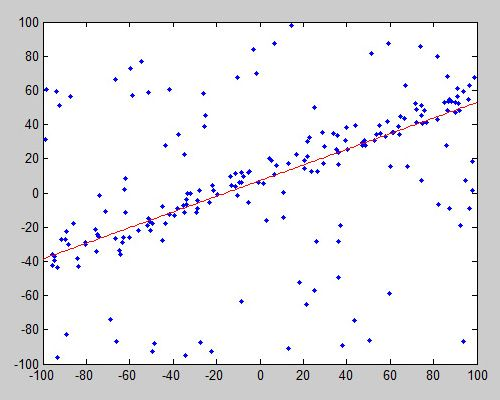
\includegraphics[width=0.8\linewidth]{assets/ransac.jpg} 
    \caption{\small Data points shown in blue, with the line of form y = mx+c estimated using RANSAC indicated in red. - \textit{https://www.mathworks.com}.}
    \label{fig:ransac}
\end{figure}

Algorithms for pattern recognition, collapse heterogeneous realities into standardized, data-driven abstractions. However, certain local specificities do not easily conform to the logic of machine learning. These \textit{"outliers"} or \textit{"anomalies"} are often treated as statistical noise, rather than meaningful divergences that could challenge the system's assumptions. Problematizing locality, then, requires acknowledging that what is excluded from modeling is not neutral but politically significant.

AI models often depend on data extracted from local contexts but are deployed in a non-localized, decontextualized manner. This reinforces structural inequalities, where data from marginalized communities is used to optimize systems that do not serve them, or actively oppress them (e.g., urban surveillance and predictive policing).

{\scriptsize \textcolor{comment}{\% Analytical acceptance, algorithmic forgiveness. }}

I went through many struggles conforming to neurotypical norms. As a child, I used to write mirrored text and had difficulty reading, so I was quickly diagnosed with dyslexia. I suffered from insomnia for a big portion of my adolescence, as a result of the discomforts of forced social interactions. Later in life, I was prescribed with medication for anxiety disorders due to unbearable panic attack seasons. I was diagnosed quite late in life with ADHD (Attention Deficit Hyperactivity Disorder), followed with a possible co-occurrence of ASD (Autism Spectrum Disorder), a mixed condition that affects a small percentage of the population\footnote{ADHD has a global prevalence of around 5-7\% of children and 2-5\% of adults. Around 20-50\% of individuals with ADHD also meet criteria for ASD.}. I started making sense of the previous 40 years, the anxiety, the insomnia, the lack of personal memories, and the depression caused by simply not fitting-in. I came to realize that a deeper knowledge and understanding of this region of the spectrum became my way of making sense of my interactions with the world, allowing me to forgive myself and others, while also developing the necessary rational arguments to actively reject the structures responsible for perpetuating the generalized norms that shape our societies.

{\scriptsize \textcolor{comment}{\% symbiotic contamination}}

In the current context of a neurotypical majority, forging the options and leading to a society that values selection over creativity, the creation of our own tools seems to be an appropriate choice to true creativity. Such practices allow to dig into deeper understanding of the final outcomes, and explore the equally rich properties of every step of a process.  

\subsection*{time scales}

For some neurodivergent individuals, time feels less sequential and more layered or interconnected, as if different dimensions of experience coexist and interact simultaneously. Moments may feel fragmented, time may be experienced in hyperfocus (expanding infinitely) or in rapid, disjointed flashes. Much like a hologram contains a vast amount of information compressed into a simpler lower-dimensional form, neurodivergent cognition could compress complex timelines and experiences into non-linear formats, creating unique interpretations and associations across time.
Neurodivergent cognition might operate by projecting internal mental states or processing vast amounts of sensory data into condensed forms like patterns, metaphors, or unique associations. 

% new:
Deleuze's concept of the \textit{"irrational cut"} in cinema\footnote{Deleuze frequently references Godard as a master of the "irrational cut"}, introduced in "\textit{Cinema 2: The Time-Image}"\citep{deleuze1985}, marks a fundamental disruption of classical continuity and logical progression in film editing. Unlike the \textit{"rational cut"} of classical cinema, which follows a clear cause-and-effect chain, the irrational cut severs this logical flow, creating temporal and spatial disjunctions that do not adhere to conventional narrative logic. Instead, these cuts generate pure time-images, where past, present, and future may coexist in ambiguous and nonlinear ways.

This disruption of linearity in cinema resonates deeply with neurodivergent modes of perception and cognition, particularly in conditions such as ADHD, autism, and certain forms of synesthesia, where experiences of time, memory, and causality often do not conform to neurotypical expectations.

Many neurodivergent individuals experience thought processes that operate in a non-hierarchical, associative, or rhizomatic manner. Rather than following a clear sequence, thoughts, memories, and perceptions may form intricate networks where disparate elements become linked without a clear rational justification. This mirrors how the irrational cut allows film sequences to be connected not through logic, but through affect, intuition, or symbolic resonance.
%  add citep 
 
{\scriptsize \textcolor{comment}{\% failures with a serial number}}

I'm interested in multi-sensory installations, layered audio-visual compositions, or interactive works that allow viewers to experience various \textit{"time slices"} of the piece, where events and emotions compress into a single moment. Experiences of layered and non-linear time are certainly an inspiration to an approach that defies linear storytelling or straightforward interaction.

{\scriptsize \textcolor{comment}{\% examples}}

In his Theater Series, Figure~\ref{fig:sugimoto}, Hiroshi Sugimoto \citep{sugimotohiroshi} created a series of long-exposure photographs of cinemas where an entire film is projected onto a single frame, collapsing a full-length movie into a single luminous image. Similarly, in Figure~\ref{fig:mv01}, a digital work of my own authorship, the equation for incremental mean calculation is implemented to run over video sequences, presenting time not as linear but as an accumulation of all its moments at once.

The generative installation titled \textit{"33 Questions per Minute"}, by Rafael Lozano-Hemmer \citep{lozano-hemmer}, Figure~\ref{fig:lozano}, shows a rapidly changing sequence of randomly generated questions on LCD screens, exceeding the speed at which they can be read. This creates a layered simultaneity of potential meanings and missed moments in time.

%% image
\begin{figure}
    \centering
    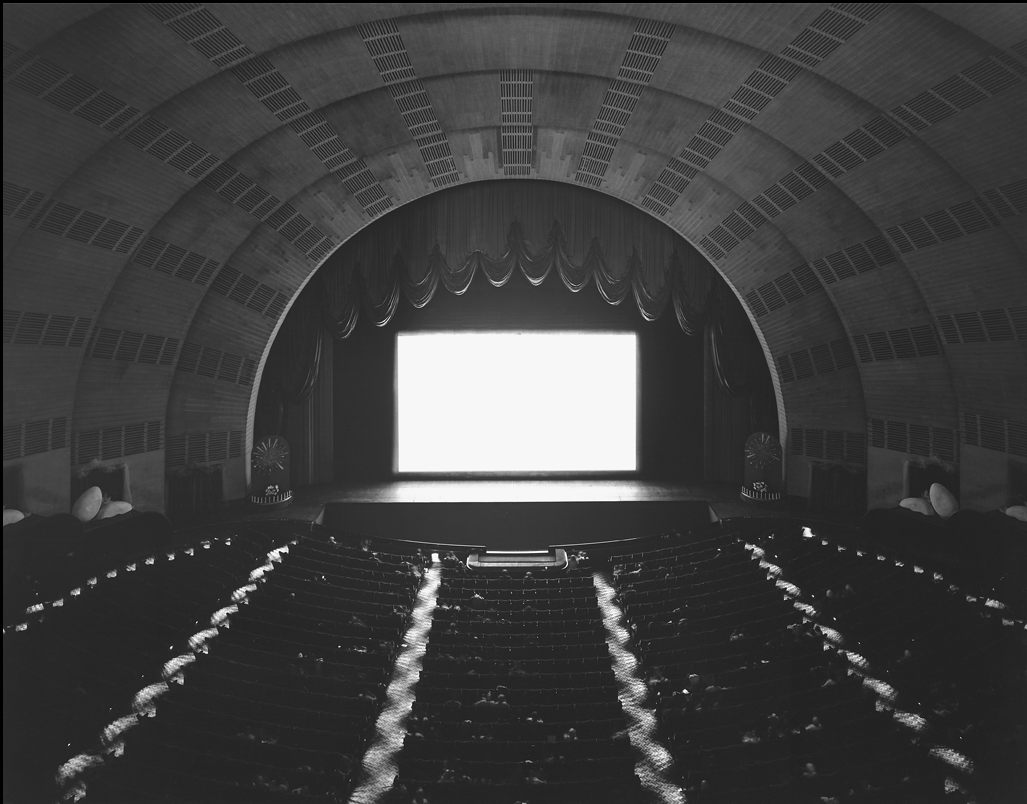
\includegraphics[width=0.8\linewidth]{assets/hiroshi-sugimoto-theaters-1978-1993-Radio-City-Music-Hall-1.png} 
    \caption{\small  Radio City Music Hall, New York 1978 - \textit{Hiroshi Sugimoto, Theaters, https://yoshiigallery.com}.}
    \label{fig:sugimoto}
\end{figure}


%% image
\begin{figure}
    \centering
    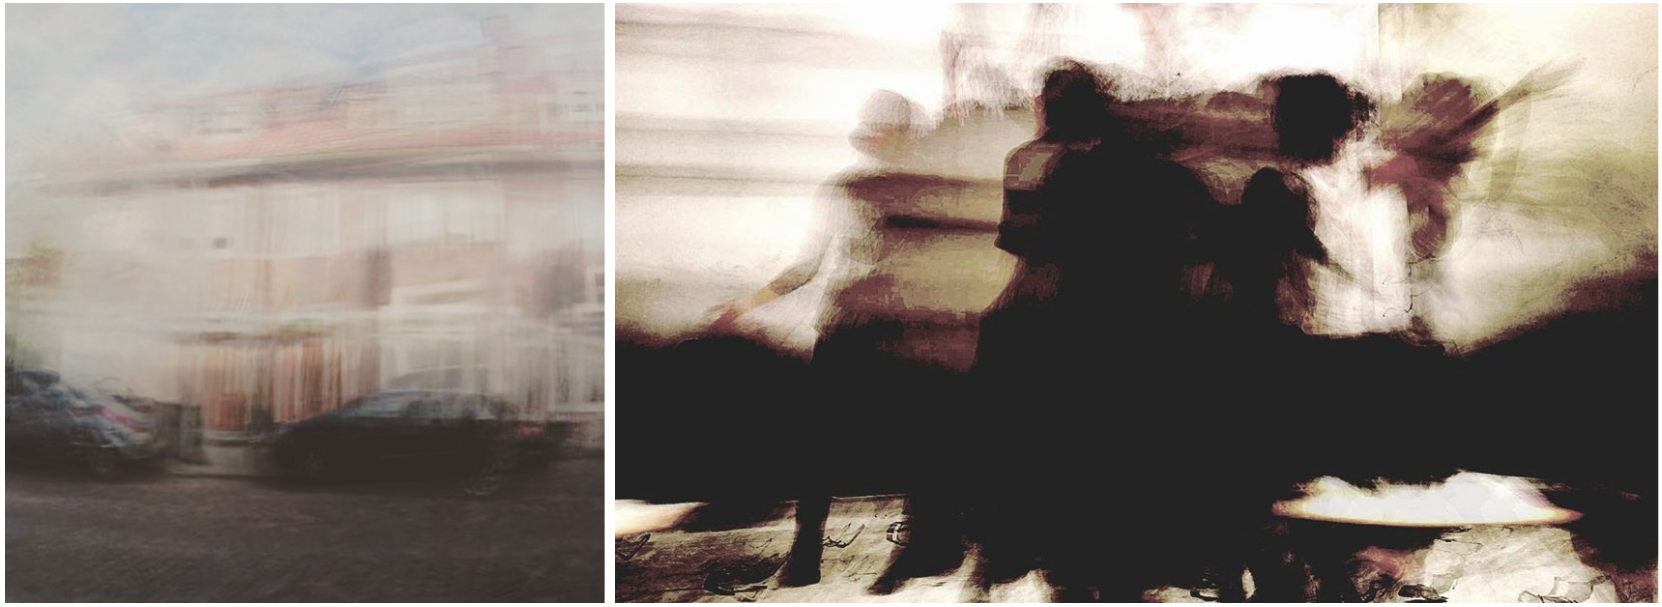
\includegraphics[width=0.8\linewidth]{assets/average.png} 
    \caption{\small \( u_{n+1} = u_{n} + \frac{x_{n+1} - u_{n}}{n+1} \) - \textit{Mauricio van der Maesen de Sombreff, video frames average}.}
    \label{fig:mv01}
\end{figure}

%% image
\begin{figure}
    \centering
    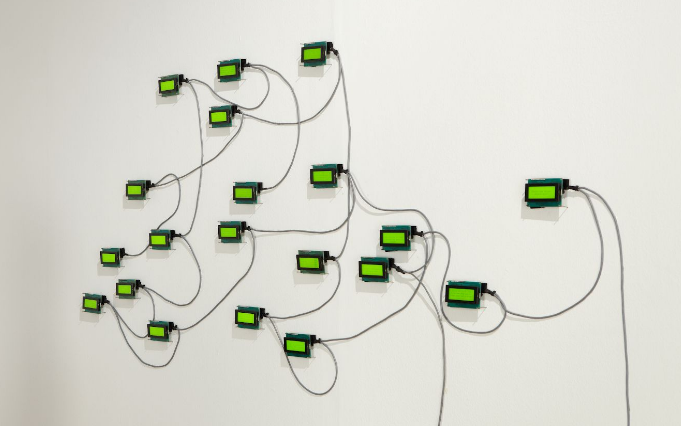
\includegraphics[width=0.8\linewidth]{assets/33_questions_per_minute_grifo.png} 
    \caption{\small Display version - \textit{Rafael Lozano-Hemmer, 33 questions per minute, https://www.lozano-hemmer.com}.}
    \label{fig:lozano}
\end{figure}



\addcontentsline{toc}{chapter}{perception}

\begin{center}
\vspace*{\fill}
\Huge{perception}

\vspace{2cm}

\begin{flushright}
\large{
\textit{Self-Organized Criticality}}
\end{flushright}

\vspace*{\fill}
\end{center}

Loud drones, low frequency soothing sounds.
Whispers louder than the loudest screams. 
A new detail that changed my day. 
The repetitive, unsettling  touch.
Tight knotts like hugs. 
Invasive gazes that were not supposed to last.
The faces, the mirrors, the shadows. 


Self-Organized Criticality describes how certain systems naturally evolve toward a critical, highly sensitive state where small changes can lead to large-scale effects. This state of criticality is "self-organized" because the system doesn’t require external tuning to reach this point. It naturally arranges itself into this state through its own dynamics. These models help describe the experience of sensory amplification, where the world can be perceived in vivid detail or with overwhelming intensity. 

\chapter*{Laplace's demon}
\addcontentsline{toc}{chapter}{Laplace's demon}

Pierre-Simon de Laplace conceived a thought experiment involving a hypothetical intelligent being with knowledge of the current state of everything and the capacity to process all that information. Under the hypothesis of a deterministic universe, such a being would know both the past and the future, thereby eliminating the perception of time, since everything that exists now would also reveal what was and what will be.

In a much more limited context of both space and time, the constant monitoring of microscopic changes and patterns places me in a position to predict possible futures and assume causality from potential pasts. I live without a normal perception of time, burdened by the overwhelming anxiety of processing all possible realities with the same intensity as the "here and now." Predicting an experience and experiencing the predictions. Presuming a cause for every effect. Speculative remembering, blurring memories.

\addcontentsline{toc}{chapter}{hypervigilance}
\begin{center}
% \vspace*{\fill}
\Huge hypervigilance
\vspace{2cm}
\begin{flushright}
\large
\textit{Stochastic resonance is a phenomenon in which a signal that is normally too weak to be detected by a sensor can be boosted by adding white noise}
\end{flushright}
\vspace{2cm}
% \vspace*{\fill}
\end{center}
\normalsize

Whenever I take a walk, I don't just stroll from A to B. I'm constantly monitoring every obstacle, every moving object and person around, everything that can be moved by the wind or shifted by the weight of raindrops. I calculate the next position of every object, adjusting my trajectory to account for the space needed for myself and my companion, when there's one by my side. I walk, and I am in the near future as much as I am in the present—more than most people I've discussed this with.

I observe what everyone else sees, and I analyze the changes in their motion patterns and facial expressions, curiously attempting to predict their intentions, possible thoughts, and probable actions. I play out their actions in my mind like a game of chess. I'm here and now, yet I am also everywhere before and after. I'm everyone in my own form, simultaneously avoiding and seeking connection.

The brain’s "signal detector" operating in an overly sensitive state, amplifies both real and perceived threats. Constant monitoring, responsiveness, attention to subtle changes, amplified details that go often unnoticed. 

{\scriptsize \textcolor{comment}{\%  How could I share a hyper-experience ?}}

\citep{wiesenfeld1995}




\addcontentsline{toc}{chapter}{Wave Function Collapse}

\begin{center}
\vspace*{\fill}
\Huge Wave Function Collapse

\vspace{2cm}

\begin{flushright}
\large
\textit{ $\text{a} \propto \text{E}$ }
\end{flushright}
\vspace*{\fill}
\end{center}

\normalsize

% This chapter talks about influences of the unknown on anxiety. 

Anxiety is proportional to the entropy of a situation. 


\subsection*{ Entropy, quantum mechanics and Sudoku solving} 

The algorithmic way to solve a sudoku puzzle, is to find the cells 
that present minimum entropy. 
This means, find the cells where the number of possible options is smaller.
When a possible solution is presented to this cell, the cells around them will 
in turn decrease their entropy. 

According to quantum mechanics, the wave function represents the probabilities 
of different coexisting realities, that is, until a 
measurement is made. At the moment of measurement, chance is replaced by 
actuality. The wave function collapses, and reality is set.

Every unknown in life, every decition still not made, creates a multitude of 
posibilities, a distribution of paralel potential realities, simultaneously 
existing in a high entropy state. 

Making a decision, or a discovery, will collapse all posibilities into one, 
reducing entropy and in consecuence reducing the asociated anxiety for the unknown. 







%\lipsum[6-10]  % Example text

\chapter*{Emulation}
\addcontentsline{toc}{chapter}{Emulation}

Living often feels like running a sophisticated emulation program on a computer. On the surface, the emulated environment mimics a typical operating system, seamlessly performing tasks and following expected protocols. However, behind this facade of normality, a complex system is working overtime to replicate behaviors and responses that come naturally to others. Constantly striving to appear organized, focused, and in control, while internally grappling with distraction, impulsivity, and a torrent of unfiltered thoughts.

Just as an emulated system can lag or crash when overloaded, I become overwhelmed and fatigued by the continuous effort to conform to neurotypical standards. The emulation requires immense mental resources, leading to burnout and a sense of disconnection from my authentic self.

\addcontentsline{toc}{chapter}{decay}

\begin{center}
\vspace*{\fill}
\Huge{decay}

\vspace{2cm}

\begin{flushright}
\large{
\textit{ n \rightarrow p^+ + e^- + \bar{\nu}_e }}
\end{flushright}

\vspace*{\fill}
\end{center}

When an atom has an unbalanced number of protons and neutrons in its nucleus, it becomes unstable. When an element is unstable, it decays. If there are additional neutrons, making the atom heavier and disrupting the internal nuclear forces, a neutron can transform into a proton by emitting an electron and an antineutrino. This type of decay is known as beta-minus decay.

Just like a carbon-14 atom, with an extra pair of neutrons, we carry the weight of indecision, of uncertainty, of forces that throw our lives out of balance. And just like that carbon atom, we decay, emitting electrons and antineutrinos—massless and imperceptible particles we leave behind, transforming. And just like the resulting nitrogen-14, older and stable, we find rest.

\renewcommand{\bibname}{references}  % Change the name of the bibliography section
\bibliographystyle{plainnat}
\bibliography{thesis}


\end{document}
